\documentclass[12pt]{article}
\usepackage{placeins}
\usepackage{sbc-template}
\usepackage{float}
\usepackage{graphicx,url}
\usepackage{listings}
\usepackage[brazil]{babel}   
%\usepackage[latin1]{inputenc}  
\usepackage[utf8]{inputenc} 
\usepackage{color}
\definecolor{dkgreen}{rgb}{0,0.6,0}
\definecolor{gray}{rgb}{0.5,0.5,0.5}
\definecolor{mauve}{rgb}{0.58,0,0.82}
 
% UTF-8 encoding is recommended by ShareLaTex
\usepackage{}
\sloppy
\lstset{
  language=Python,                
  basicstyle=\footnotesize,           
  numbers=left,                   
  numberstyle=\tiny\color{gray},  
  stepnumber=2,                             
  numbersep=5pt,                  
  backgroundcolor=\color{white},    
  showspaces=false,               
  showstringspaces=false,         
  showtabs=false,                 
  frame=single,                   
  rulecolor=\color{black},        
  tabsize=2,                      
  captionpos=b,                   
  breaklines=true,                
  breakatwhitespace=false,        
  title=\lstname,                               
  keywordstyle=\color{blue},          
  commentstyle=\color{dkgreen},       
  stringstyle=\color{mauve}, }

\title{Segundo Projeto de Comunicações Móveis}

\author{Vítor Gabriel Lemos Lopes}


\address{Departamento de Engenharia de Comunicações-UFRN
}

\begin{document} 

\maketitle

     
\begin{resumo} 
  Este Trabalho foi feito com intuito de modelagem de um sistema WCDMA com reuso 1, para podermos observar a interferência que cada usuário causa em seus vizinhos. Dado os códigos em matlab, foi feito uma tradução dos códigos de matlab para python e foram feitas algumas modificações para poder funcionar.
\end{resumo}
 
\section{\huge 8.1} \label{sec:firstpage}
Foi pedido para que fosse gerado um gráfico com o grid das 7 células com com 1000 usuários em cada célula.
\begin{figure}[h]
    \centering
    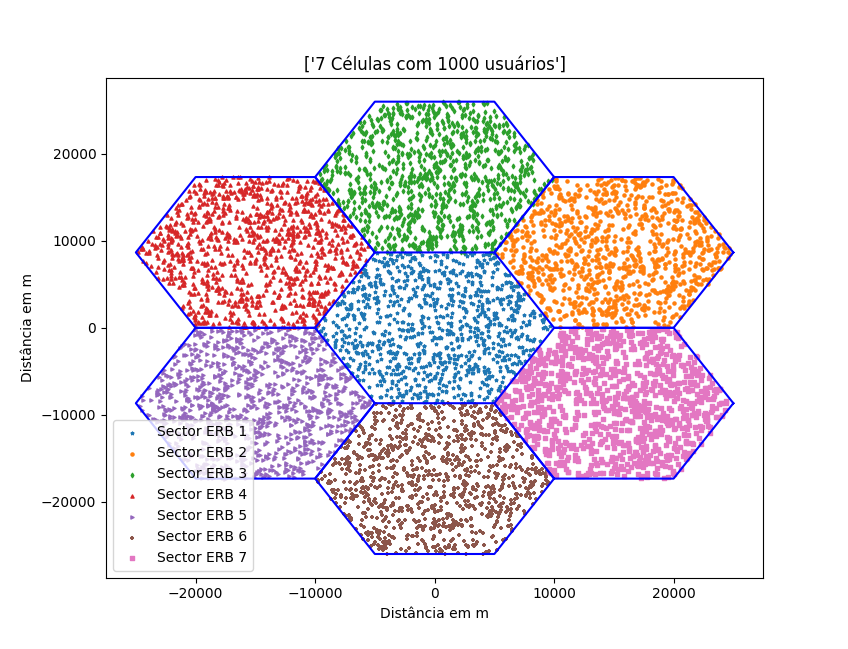
\includegraphics[width=1\textwidth]{GridQ1.png}
    \caption{Grid para 1000 usuários}
    \label{fig:my_label}
\end{figure}

\section{\huge 8.2}

Foi pedido para que fosse gerado as CDFs da Eb/No, potência transmitida e potência recebida para os raios de  50, 100, 500, 2000 e 10000 metros, com uma quantidade de usuários de 200.
\begin{figure}[h]
    \centering
    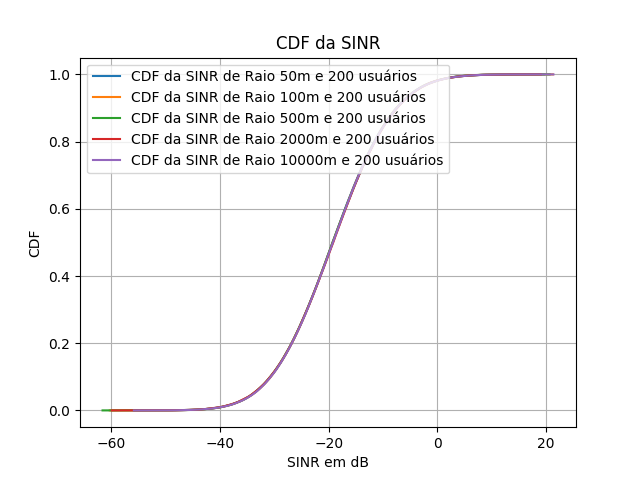
\includegraphics[width=0.75\textwidth]{SINRQ2.png}
    \caption{CDF Eb/No}
    \label{fig:my_label}
\end{figure}
\begin{figure}[h]
    \centering
    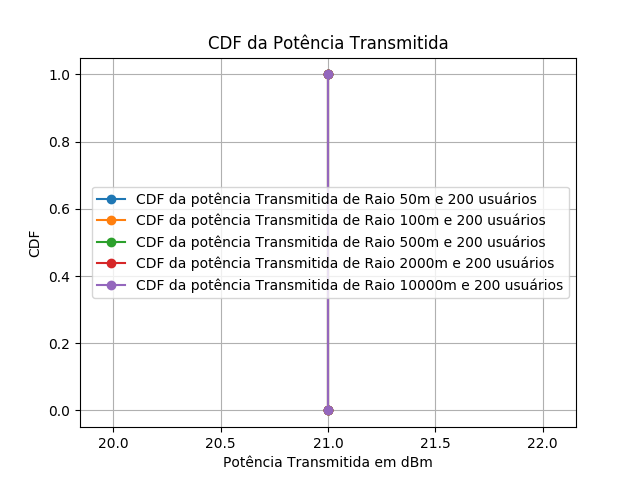
\includegraphics[width=0.65\textwidth]{PTQ2.png}
    \caption{CDF Potência Transmitida}
    \label{fig:my_label}
\end{figure}
\begin{figure}[h]
    \centering
    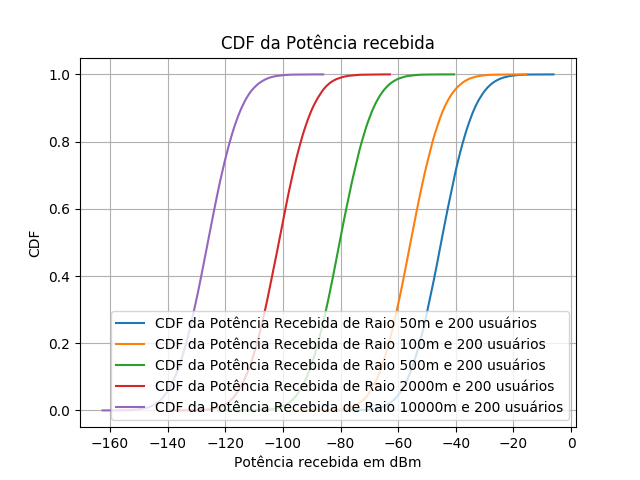
\includegraphics[width=0.75\textwidth]{PRQ2.png}
    \caption{CDF Potência Recebida}
    \label{fig:my_label}
\end{figure}
\FloatBarrier
Com os Gráficos gerados podemos observar as seguintes coisas:\\
A a Eb/No continua a mesma na média para vários raios, porque a interferência dos outros usuários influenciam na mesma proporção de raios pequenos e com raios grandes, se a potência recebida naquele ponto é alta, a interferência dos que estão próximas também vão ser altas. \\
A potência recebida na ERB é maior para os os usuários mais próximos do que para os que estão nas bordas, devido a perda de percurso.\\
A potência transmitida não muda, não importa o raio ou a quantidade de usuários, porque cada usuário vai transmitir na mesma potência.\\
A potência recebida vai aumentado de acordo com o valor do raio, devido a perda de percurso ser menor.
\section{\huge 8.3}
Foi pedido para que fosse gerado as CDFs da Eb/No e potência recebida para os raios de  50, 100, 500, 2000 e 10000 metros, com uma quantidade de usuários de 10.
\begin{figure}[h]
    \centering
    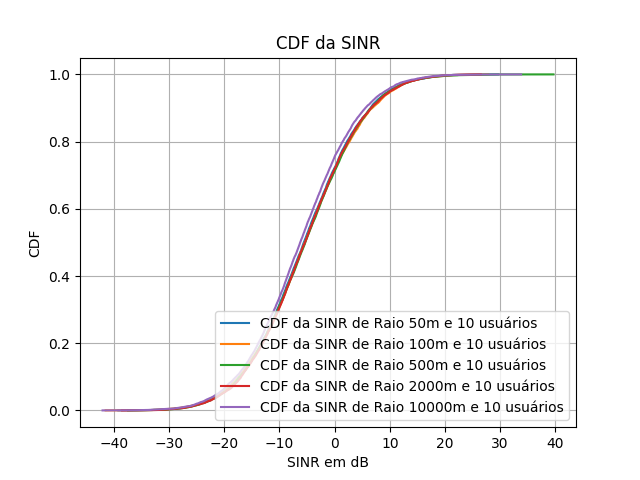
\includegraphics[width=0.75\textwidth]{SINRQ3.png}
    \caption{CDF Eb/No}
    \label{fig:my_label}
\end{figure}
\FloatBarrier
\begin{figure}[h]
    \centering
    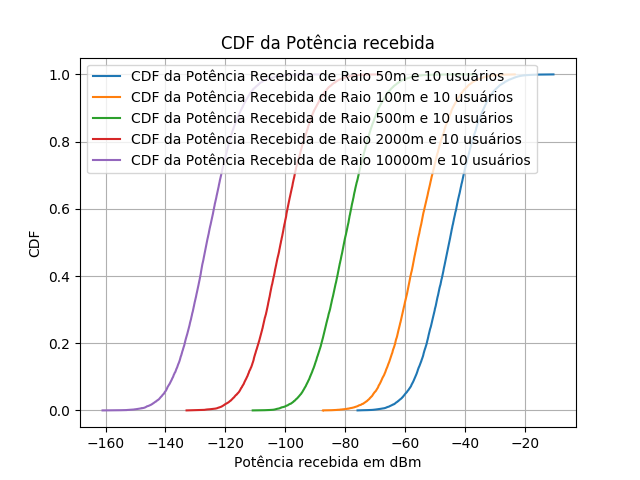
\includegraphics[width=0.75\textwidth]{PRQ3.png}
    \caption{CDF Potência Recebida}
    \label{fig:my_label}
\end{figure}
\FloatBarrier
Com estes gráficos podemos observar:

A Eb/No fica muito próxima, mas não fica exatamente uma em cima da outra, porque a quantidade de usuários é muito pequena mas como é proporcional, ela ainda fica muito próxima uma da outra, acontece também que ela ganha cerca de 20dB de diferença do que tem 200 usuários, fica com menor interferência .\\
A potência recebida não é afetada pela quantidade de usuários e apenas pelo raio devido a perda de percurso.\\
A única formulação que explica esse comportamento é a formula de transformação de energia, de Watt para escala logarítmica. 

\section{\huge 8.4}
Foi pedido para que fosse gerado as CDFs da Eb/No, potência transmitida e potência recebida para o raio de 100 metros, com uma quantidade de usuários de 10,50,200 e 1000.
\begin{figure}[h]
    \centering
    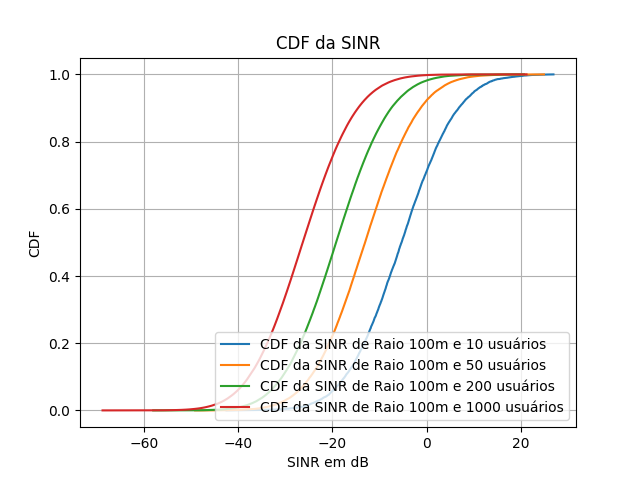
\includegraphics[width=1\textwidth]{SINRQ4.png}
    \caption{CDF Eb/No}
    \label{fig:my_label}
\end{figure}
\begin{figure}[h]
    \centering
    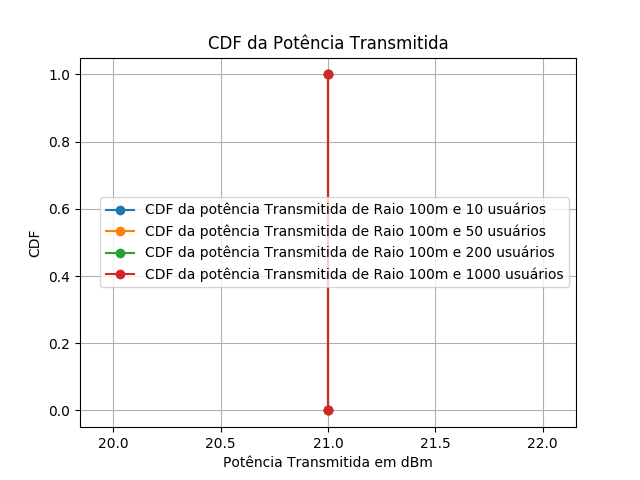
\includegraphics[width=0.75\textwidth]{PTQ4.png}
    \caption{CDF Potência Transmitida}
    \label{fig:my_label}
\end{figure}
\begin{figure}[h]
    \centering
    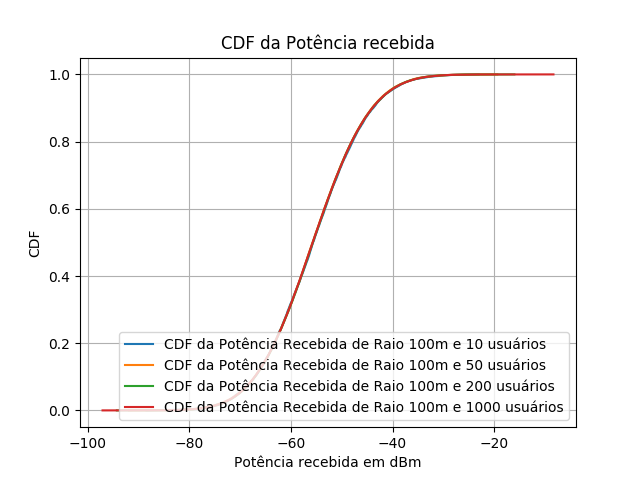
\includegraphics[width=0.75\textwidth]{PRQ4.png}
    \caption{CDF Potência Recebida}
    \label{fig:my_label}
\end{figure}
\FloatBarrier
Com os Gráficos gerados podemos observar as seguintes coisas:\\
A quantidade de usuários influenciam no Eb/No, porque quanto maior a quantidade de usuários, maior será a interferência. \\
A quantidade de usuários afeta igualmente os usuários da borda e do centro porque a interferência vai ser a mesma para cada quantidade de usuários.\\
A potência recebida continua a mesma, por causa que o que influencia a potência recebida é apenas a perda de percurso que é dado pelo raio da célula. 
%\bibliographystyle{sbc}
%\bibliography{sbc-template}
\section{\huge 8.5}
Para o raio de cobertura de 90\% é de valor entre 3350 e 3500 metros, essa variação é devida ao sombreamento que também afeta a potência recebida.
\section{\huge 8.6}
O sistema é limitado devido a perda de percurso e sombreamento, ou seja, quanto maior o raio mais usuários não vão ter a potência miníma para a transmissão.
\end{document}
